\documentclass{beamer}
\usetheme{metropolis}
\usepackage{graphicx}
\usepackage{subfig}
\usepackage{tcolorbox}
\title{Algebra-Based Physics: Electricity, Magnetism, and Modern Physics (PHYS135B): Unit 0}
\author{Jordan Hanson}
\institute{Whittier College Department of Physics and Astronomy}

\begin{document}
\maketitle

\section{Summary}

\begin{frame}{Unit 0 Summary}
\textbf{Reading: Chapters 3.1 - 3.3, 18.1 - 18.5, 19.1 - 19.3}
\begin{enumerate}
\item Estimation/Approximation
\item Coordinates and Vectors
\item Review of concepts from Newtonian mechanics
\begin{itemize}
\item Kinematics and Newton's Laws
\item Work-energy theorem, energy conservation
\item Momentum, conservation of momentum
\end{itemize}
\item Electrostatics I: charges and fields
\item Electrostatics II: potential, and potential energy
\end{enumerate}
\end{frame}

\section{Estimation/Approximation}

\begin{frame}{Estimation/Approximation}
In science and engineering, \alert{estimation} is to obtain a quantity in the absence of precision, informed by rational constraints.
\begin{enumerate}
\item \textbf{Define relevant \alert{unit scales}}: (mg, g, or kg), (m/s or km/hr)
\item \textbf{Obtain \alert{complex quantities}} from simple ones
\begin{itemize}
\item Obtain \textit{areas} and \textit{volumes} from \textit{lengths}
\item Obtain \textit{rates} from \textit{numerators} and \textit{denominators}
\end{itemize}
\item \textbf{Taking advantage of \alert{scaling problems}}
\begin{itemize}
\item Knowing \textit{relationship} between variables
\item Using that \textit{relationship} to obtain new information
\end{itemize}
\item \textbf{Constrain the unknown with \alert{upper} and \alert{lower} limits}
\end{enumerate}
\end{frame}

\begin{frame}{Estimation/Approximation}
\textbf{Unit scale}: A generation is about one-third of a lifetime. Determine how many generations have passed since the year 0 AD\footnote{What is the appropriate scale here?}.
\begin{itemize}
\item A: $10$
\item B: $20$
\item C: $60$
\item D: $100$
\end{itemize}
\end{frame}

\begin{frame}{Estimation/Approximation}
\textbf{Unit scale}: (a) What fraction of Earth’s diameter\footnote{The diameter of the Earth is 12,800 km.} is the greatest ocean depth (11 km below sea level)? (b) The greatest mountain height (8.8 km above sea level)?
\begin{itemize}
\item A: $8.6 \times 10^{-2}$, $6.9 \times 10^{-2}$
\item B: $8.6 \times 10^{-3}$, $6.9 \times 10^{-3}$
\item C: $8.6 \times 10^{-4}$, $6.9 \times 10^{-4}$
\item D: $8.6 \times 10^{-5}$, $6.9 \times 10^{-3}$
\end{itemize}
\end{frame}

\begin{frame}{Estimation/Approximation}
\textbf{Complex quantities}: Assuming one nerve impulse must end before another can begin, what is the maximum firing rate of a nerve in impulses per second? 
\begin{itemize}
\item A: 1 per second (1 Hz)
\item B: 30 per second (30 Hz)
\item C: 60 per second (60 Hz)
\item D: 100 per second (100 Hz)
\end{itemize}
\end{frame}

\begin{frame}{Estimation/Approximation}
\textbf{Complex quantities}: If a Whittier College athlete ran the 5k race at a track meet in 35 minutes, what was her average speed?
\begin{itemize}
\item A: 0.3 meters per second
\item B: 3 meters per second
\item C: 30 meters per second
\item D: 300 meters per second
\end{itemize}
\end{frame}

\begin{frame}{Estimation/Approximation}
\textbf{Complex quantities}: Suppose you won the lottery and received \$1 billion USD.  Because your life is dope, you stack that paper over the Whittier College soccer field.  Each stack contains 100 bills, and each bill is worth \$100.  If you evenly cover the field, how high is the money level?
\begin{itemize}
\item A: 0.5 inch
\item B: 1 inch
\item C: 2 inches
\item D: 1 foot
\end{itemize}
\end{frame}

\begin{frame}{Estimation/Approximation}
\textbf{Scaling problem}: Supposed you have an ideal gas in a cylinder of fixed volume.  If the pressure begins as 100 kPa, and you \textit{double} the temperature of the gas, what is the new pressure?
\begin{itemize}
\item A: 100 kPa
\item B: 50 kPa
\item C: 10 kPa
\item D: 200 kPa
\end{itemize}
\end{frame}

\begin{frame}{Estimation/Approximation}
\textbf{Scaling problem}: Supposed you have an ideal gas in a cylinder of fixed volume.  If the pressure begins as 100 kPa, and you \textit{halve} the temperature of the gas, what is the new pressure?
\begin{itemize}
\item A: 100 kPa
\item B: 50 kPa
\item C: 10 kPa
\item D: 200 kPa
\end{itemize}
\end{frame}

\begin{frame}{Estimation/Approximation}
\textbf{Upper/lower limits}: How many undergraduate students are there at Whittier College\footnote{What is the absolute lower limit, and what is the upper limit?}?
\begin{itemize}
\item A: 5,000
\item B: 1,000
\item C: 1,250
\item D: 500
\end{itemize}
\end{frame}

\begin{frame}{Estimation/Approximation}
\textbf{Upper/lower limits}: What is the average yearly college tuition in the United States (before subtracting grants and scholarships)?
\begin{itemize}
\item A: \$5,000
\item B: \$10,000
\item C: \$25,000
\item D: \$40,000
\end{itemize}
What information affects the \alert{upper} and \alert{lower} limits here?
\end{frame}

\section{Coordinates and Vectors}

\begin{frame}{Coordinates and Vectors (Chapters 3.1 - 3.3)}
Physics requires \alert{mathematical objects} to build equations that capture the behavior of nature.  Two examples of such objects are \alert{scalar} and \alert{vector} quantities.  Each type of object obeys similar but different rules.
\begin{enumerate}
\item Scalar quantities
\begin{itemize}
\item mass: $m_1+(m_2+m_3) = (m_1+m_2)+m_3$
\item speed: $v_1(v_2+v_3) = v_1v_2+v_1v_3$
\item charge: $q_1 \left(\frac{1}{q_1}\right) = 1$, $q_1(0) = 0$
\end{itemize}
\item Vector quantities
\begin{itemize}
\item velocity: $\vec{v}_1 + (\vec{v}_2+\vec{v}_3) = (\vec{v}_1 + \vec{v}_2)+\vec{v}_3$
\item tension: $\vec{t}_1 \cdot (\vec{t}_2 + \vec{t}_3) = \vec{t}_1 \cdot \vec{t}_2 + \vec{t}_1 \cdot \vec{t}_3$
\end{itemize}
\end{enumerate}
\textbf{Examples: break into components, adding two vectors.}
\end{frame}

\begin{frame}{Coordinates and Vectors (Chapters 3.1 - 3.3)}
A vector may be expressed as \textit{a list of scalars}: $\vec{v} = (4,2)$ (a vector with two \textit{components}), $\vec{u} = (3,4,5)$ (three \textit{components}).  Now, we know how to add and subtract scalars.  How do we add and subtract vectors? \\
\vspace{0.5cm}
What is\\
$(1,3,8)+$\\ $(0,2,1)$? \\
Answer: $(1,5,9)$ \\
\vspace{0.5cm}
In other words, when adding vectors, we add them component by component. \textbf{Work several examples.}
\end{frame}

\begin{frame}{Coordinates and Vectors (Chapters 3.1 - 3.3)}
How do we subtract vectors? In the same fashion:\\
\vspace{0.5cm}
What is\\
$(1,3,8)-$\\ $(0,2,1)$? \\
Answer: $(1,1,7)$ \\
\vspace{0.5cm}
In other words, when subtracting vectors, we subtract them component by component. \textbf{Work several examples.}
\end{frame}

\begin{frame}{Coordinates and Vectors (Chapters 3.1 - 3.3)}
How do we multiply vectors? In the same fashion, \textit{for one kind of multiplication}:\\
\vspace{0.5cm}
What is\\
$(1,3,8)\cdot (0,2,1)$? \\
Answer: $1\cdot 0 + 3 \cdot 2 + 8 \cdot 1 = 14$ \\
\vspace{0.5cm}
\textit{This kind of multiplication is known as the dot-product}.  There is also the \textit{cross-product}, which we will save for later. \textbf{Work several examples.}
\end{frame}

\begin{frame}{Coordinates and Vectors (Chapters 3.1 - 3.3)}
\small
The components of a vector may describe quantities in a \alert{coordinate system}, such as \textit{Cartesian coordinates} - after Ren\'e Descartes.  Vectors in the 3D Cartesian coordinate system (x,y,z) may be written in the following notation:
\\
\vspace{0.2cm}
$\boxed{\vec{v} = a\hat{i} + b\hat{j} + c\hat{k}}$
\\
\begin{itemize}
\item a: The amount in the +x-direction, $\hat{i}$: a vector of length 1, in the +x-direction
\item b: The amount in the +y-direction, $\hat{j}$: a vector of length 1, in the +y-direction
\item c: The amount in the +z-direction, $\hat{k}$: a vector of length 1, in the +z-direction
\end{itemize}
\end{frame}

\begin{frame}{Coordinates and Vectors (Chapters 3.1 - 3.3)}
\begin{figure}
\centering
\subfloat[\label{fig:twovectors_a}]{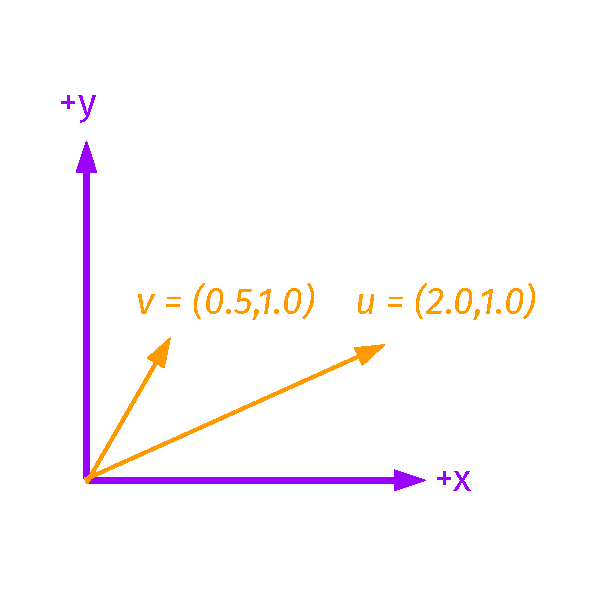
\includegraphics[width=0.45\textwidth,trim=1cm 1cm 1cm 1cm,clip=true]{figures/Vectors1.pdf}}
\subfloat[\label{fig:twovectors_b}]{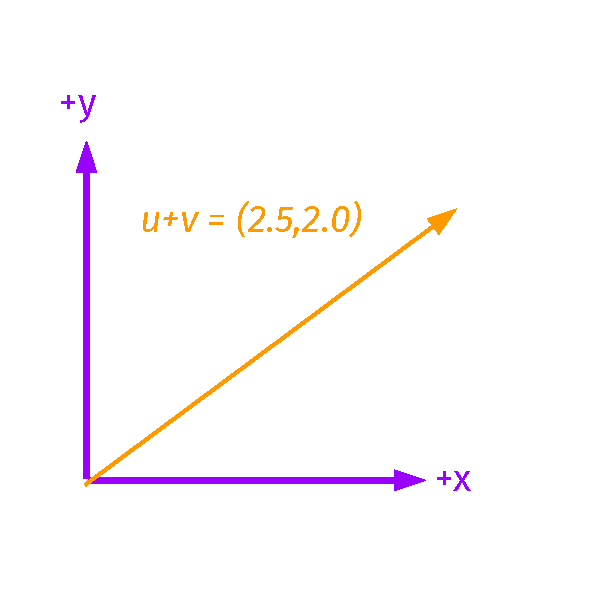
\includegraphics[width=0.45\textwidth,trim=1cm 1cm 1cm 1cm,clip=true]{figures/Vectors2.pdf}}
\caption{\label{fig:twovectors} (a) Two vectors in a two-dimensional Cartesian coordinate system: $\vec{u} = 0.5\hat{i}+1.0\hat{j}$ and $\vec{v} = 2.0\hat{i}+1.0\hat{j}$.  (b) What is $\vec{u}+\vec{v}$?  Adding components: $\vec{u}+\vec{v} = 2.5\hat{i}+2.0\hat{j}$.}
\end{figure}
\end{frame}

\begin{frame}{Coordinates and Vectors (Chapters 3.1 - 3.3)}
\begin{figure}
\centering
\subfloat[\label{fig:twovectors_c}]{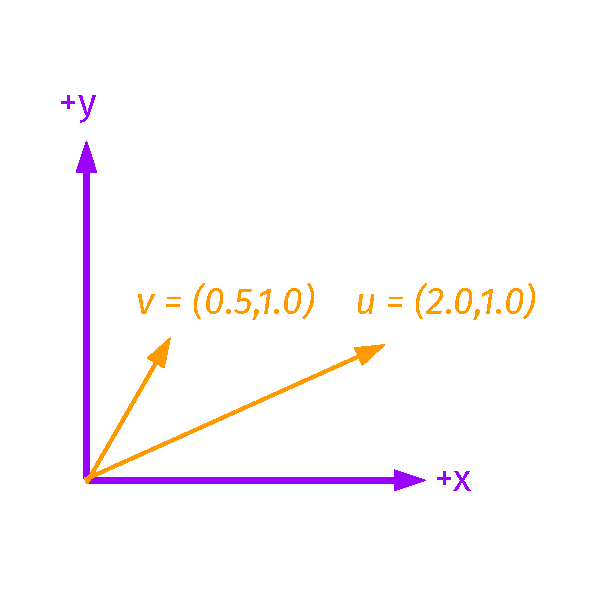
\includegraphics[width=0.45\textwidth,trim=1cm 1cm 1cm 1cm,clip=true]{figures/Vectors1.pdf}}
\subfloat[\label{fig:twovectors_d}]{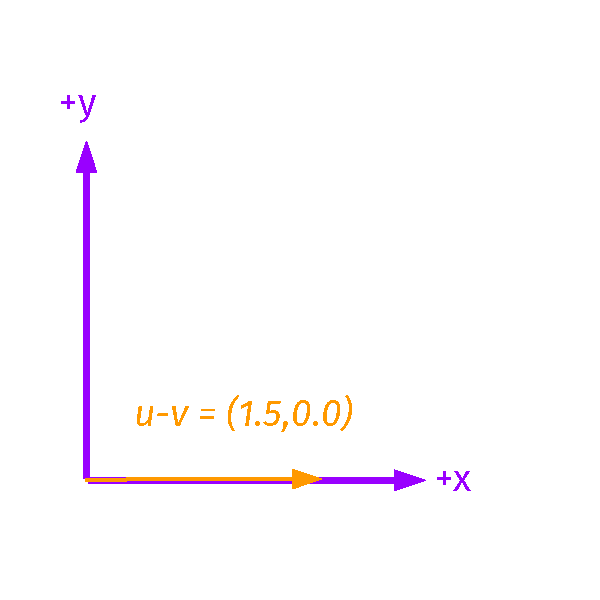
\includegraphics[width=0.45\textwidth,trim=1cm 1cm 1cm 1cm,clip=true]{figures/Vectors3.pdf}}
\caption{\label{fig:twovectors2} (a) Two vectors in a two-dimensional Cartesian coordinate system: $\vec{u} = 0.5\hat{i}+1.0\hat{j}$ and $\vec{v} = 2.0\hat{i}+1.0\hat{j}$.  (b) What is $\vec{u}-\vec{v}$?  Subtracting components: $\vec{u}-\vec{v} = 1.5\hat{i}+0.0\hat{j}$.}
\end{figure}
\end{frame}

\begin{frame}{Coordinates and Vectors (Chapters 3.1 - 3.3)}
\begin{figure}
\centering
\subfloat[\label{fig:twovectors_e}]{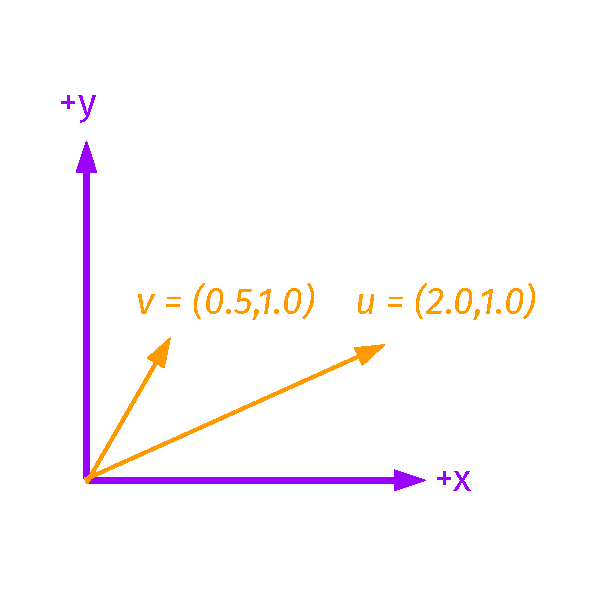
\includegraphics[width=0.45\textwidth,trim=1cm 1cm 1cm 1cm,clip=true]{figures/Vectors1.pdf}}
\subfloat[\label{fig:twovectors_f}]{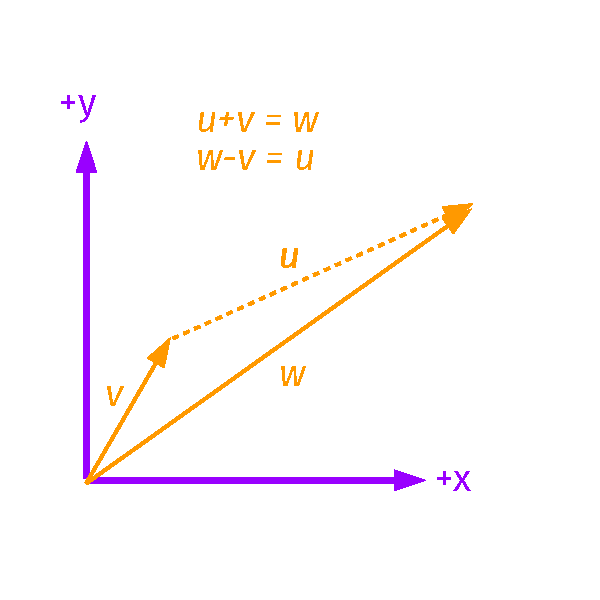
\includegraphics[width=0.45\textwidth,trim=1cm 1cm 1cm 1cm,clip=true]{figures/Vectors4.pdf}}
\caption{\label{fig:twovectors3} (a) Two vectors in a two-dimensional Cartesian coordinate system: $\vec{u} = 0.5\hat{i}+1.0\hat{j}$ and $\vec{v} = 2.0\hat{i}+1.0\hat{j}$.  (b) To compute $\vec{w}-\vec{v}$, arrange the vectors to get a sense of the result, $\vec{u}$.}
\end{figure}
\end{frame}

\begin{frame}{Coordinates and Vectors (Chapters 3.1 - 3.3)}
\small
\begin{minipage}[b]{0.45\linewidth}
Suppose $\vec{x}_i = -3\hat{i} + 2\hat{j}$ km, and $\vec{x}_f = -3\hat{i} - 2\hat{j}$ km.  What is the \textit{displacement}?
\vspace{0.2cm}
\begin{itemize}
\item A: $4\hat{i}$ km
\item B: $-4\hat{i}$ km
\item C: $4\hat{j}$ km
\item D: $-4\hat{j}$ km
\end{itemize}
\end{minipage}
\hspace{0.5cm}
\begin{minipage}[b]{0.45\linewidth}
Suppose $\vec{x}_i = 3\hat{i} - 2\hat{j}$ km, and $\vec{x}_f = 3\hat{i} - 2\hat{j}$ km.  What is the \textit{displacement}?
\vspace{0.2cm}
\begin{itemize}
\item A: 0 km
\item B: $0\hat{i} + 0\hat{j}$ km
\item C: $1\hat{i}$ km
\item D: $1\hat{j}$ km
\end{itemize}
\end{minipage}
\end{frame}

\begin{frame}{Coordinates and Vectors (Chapters 3.1 - 3.3)}
We define the \textit{position} of an object as a vector locating it in a given coordinate system.  The scalar \textit{distance} is the norm of the position vector, that is, the distance to to the origin. \\
\vspace{0.5cm}
Now we can introduce the concept of \alert{displacement}: a vector describing a movement of an object.
\end{frame}

\begin{frame}{Coordinates and Vectors (Chapters 3.1 - 3.3)}
\begin{figure}
\centering
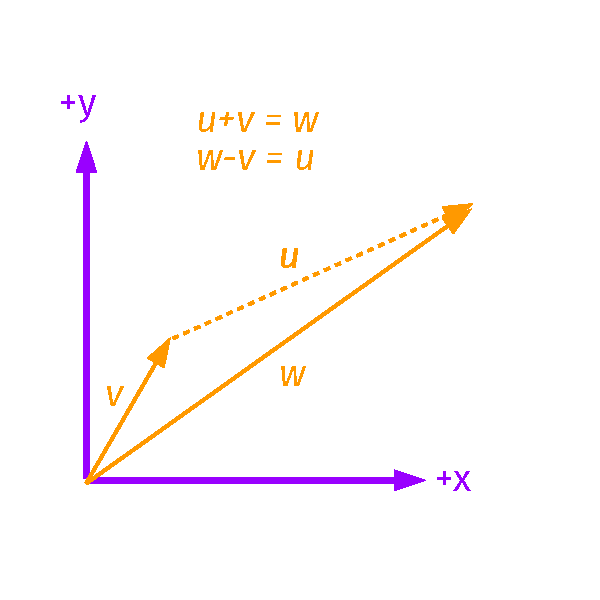
\includegraphics[width=0.52\textwidth]{figures/Vectors4.pdf}
\caption{\label{fig:displacement} Suppose an object moves from position $\vec{v}$ to $\vec{w}$.  In this case, the \alert{displacement} is $\vec{u}$. \textbf{Thus, the final position is the initial position, plus the displacement.}}
\end{figure}
\end{frame}

\begin{frame}{Coordinates and Vectors (Chapters 3.1 - 3.3)}
It follows that the \textit{displacement} is zero if the initial and final positions are the same, but the \textit{distance travelled} is not.\\
\vspace{0.2cm}
\small
Suppose a jet fighter travelling at 800 km per hour banks such that it flies in a circle of radius 0.5 km.  How long does it take to complete the circle?  What is the distance traveled, and what is the displacement?
\begin{itemize}
\item A: $2\pi$ km, 28 seconds, $2\pi$ km
\item B: $\pi$ km, 14 seconds, $\pi$ km
\item C: $\pi$ km, 28 seconds, $\pi$ km
\item D: $\pi$ km, 14 seconds, $0$ km
\end{itemize}
\end{frame}

\begin{frame}{Coordinates and Vectors (Chapters 3.1 - 3.3)}
\alert{Average velocity} is the ratio of the \alert{displacement} to the elapsed time.\\
\begin{equation}
\boxed{\vec{v}_{\rm avg} = \frac{\Delta \vec{x}}{\Delta t}}
\end{equation}
The \textit{average speed} is the norm of the average velocity:
\begin{equation}
\boxed{v_{\rm avg} = \frac{|\Delta \vec{x}|}{\Delta t}}
\end{equation}
If the motion is in one dimension, then the average speed is
\begin{equation}
v_{\rm avg} = \frac{x_{\rm f} - x_{\rm i}}{t_{\rm f} - t_{\rm i}}
\end{equation}
\end{frame}

\begin{frame}{Coordinates and Vectors (Chapters 3.1 - 3.3)}
\small
\begin{minipage}[b]{0.45\linewidth}
$\vec{p} = 4\hat{i}+2\hat{j}$.  $\vec{q} = -4\hat{i}+2\hat{j}$.  \\
Compute $\vec{p} \cdot \vec{q}$.
\vspace{0.2cm}
\begin{itemize}
\item A: 12
\item B: -12
\item C: 4
\item D: 8
\end{itemize}
\end{minipage}
\hspace{0.5cm}
\begin{minipage}[b]{0.45\linewidth}
$\vec{p} = -1\hat{i}+6\hat{j}$.  $\vec{q} = 3\hat{i}+0.5\hat{j}$.  \\
Compute $\vec{p} \cdot \vec{q}$.
\vspace{0.2cm}
\begin{itemize}
\item A: -1
\item B: 1
\item C: 0
\item D: 3
\end{itemize}
\end{minipage}
\end{frame}

\begin{frame}{Coordinates and Vectors (Chapters 3.1 - 3.3)}
Why was the last answer zero?  Look at it graphically:
\begin{figure}
\centering
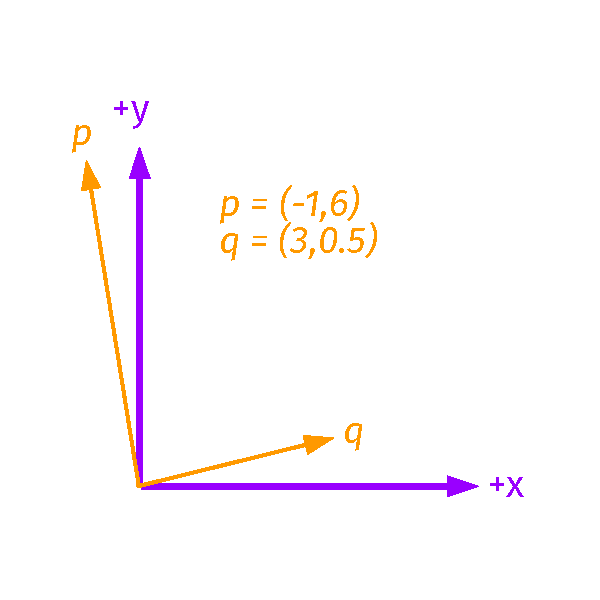
\includegraphics[width=0.5\textwidth,trim=1cm 1cm 1cm 1cm,clip=true]{figures/Vectors5.pdf}
\caption{\label{fig:twovectors4} Two vectors $\vec{p}$ and $\vec{q}$ are \textit{orthogonal} if $\vec{p} \cdot \vec{q} = 0$.}
\end{figure}
\end{frame}

\begin{frame}{Coordinates and Vectors (Chapters 3.1 - 3.3)}
The \textit{length} or \textit{norm} of a vector $\vec{v} = a\hat{i}+b\hat{j}$ is $|\vec{v}| = \sqrt{a^2+b^2}$.\\
\begin{figure}
\centering
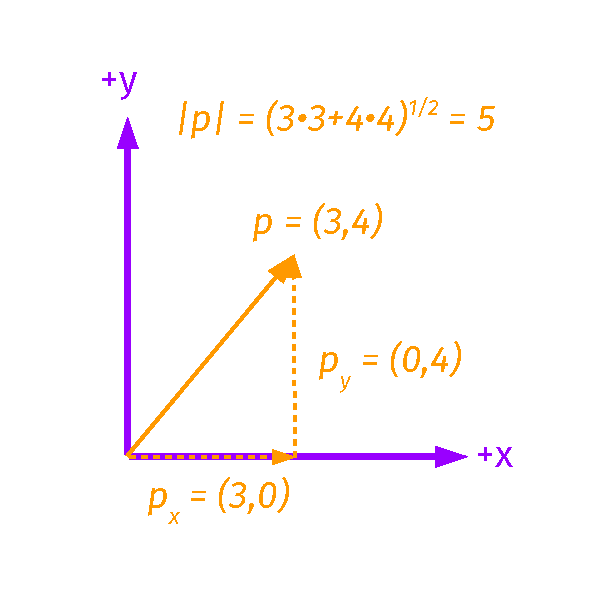
\includegraphics[width=0.5\textwidth,trim=1cm 1cm 1cm 1cm,clip=true]{figures/Vectors7.pdf}
\caption{\label{fig:twovectors6} Computing the norm of a vector $\vec{p}$.}
\end{figure}
\end{frame}

\begin{frame}{Coordinates and Vectors (Chapters 3.1 - 3.3)}
Notice that $\sqrt{\vec{p}\cdot\vec{p}} = |\vec{p}|$.\\
Let $\theta_p$ be the angle between $\vec{p}$ and the x-axis.  \\
$p_{x} = \vec{p} \cdot \hat{i} = |\vec{p}| \cos(\theta_{p})$. \\
$p_{y} = \vec{p} \cdot \hat{j} = |\vec{p}| \sin(\theta_{p})$.\\
\vspace{0.5cm}
\textit{Theorem:} The dot product of two vectors $\vec{p}$ and $\vec{q}$ is $|u||v|\cos(\theta)$, if $\theta$ is the angle between them.\\
\vspace{0.5cm}
\textit{Proof}: $\vec{p}\cdot\vec{q} = p_{x}q_{x} + p_{y}q_{y} = |p||q|\cos\theta_p\cos\theta_q+|p||q|\sin\theta_q\sin\theta_q$ \\
$=|p||q|(\cos\theta_p\cos\theta_q+\sin\theta_p\sin\theta_q) = |p||q|\cos(\theta_p-\theta_q)$ \\
$=|p||q|\cos\theta$. \\
\vspace{0.1cm}
$\boxed{\vec{p}\cdot\vec{q}=|p||q|\cos\theta}$
\end{frame}

\begin{frame}{Coordinates and Vectors (Chapters 3.1 - 3.3)}
\small
\begin{minipage}[b]{0.45\linewidth}
An object moves at 2 m/s at $\theta = 60^{\circ}$ with respect to the x-axis.  What is the velocity of the object?
\vspace{0.2cm}
\begin{itemize}
\item A: $(1\hat{i}$ + $1\hat{j})$  m/s
\item B: $(\sqrt{3}\hat{i}$ + $1\hat{j})$  m/s
\item C: $(\sqrt{3}\hat{i}$ + $\sqrt{3}\hat{j})$  m/s
\item D: $(1\hat{i}$ + $\sqrt{3}\hat{j})$  m/s
\end{itemize}
\end{minipage}
\hspace{0.5cm}
\begin{minipage}[b]{0.45\linewidth}
An object moves at 2 m/s at $\theta = 120^{\circ}$ with respect to the x-axis.  What is the velocity of the object?
\vspace{0.2cm}
\begin{itemize}
\item A: $(-1\hat{i} + \sqrt{3}\hat{j})$ m/s
\item B: $(1\hat{i} - \sqrt{3}\hat{j})$ m/s
\item C: $(-1\hat{i} + \sqrt{3}\hat{j})$ m/s
\item D: $(-1\hat{i} - \sqrt{3}\hat{j})$ m/s
\end{itemize}
\end{minipage}
\end{frame}

\begin{frame}{Coordinates and Vectors (Chapters 3.1 - 3.3)}
Is it possible to multiply vectors and scalars?  Of course: $a_1\vec{p} = a_1p_x\hat{i}+a_1p_y\hat{j}$.\\
\vspace{0.2cm}
Also, multiplication properties still hold.  For example: $(a_1+a_2)\vec{p} = a_1\vec{p}+a_2\vec{p}$. \\
\vspace{0.2cm}
\small
A spacecraft moves at 400 m/s, at an angle of 30 degrees with respect to the x-axis.  If it fires two thrusters that boost the x-component and y-component of the velocity by 25\% and 50\%, respectively, what is the final velocity?
\begin{itemize}
\item A: $(433\hat{i}+300\hat{j})$ m/s
\item B: $(300\hat{i}+433\hat{j})$ m/s
\item C: 400 m/s
\item D: $(400\hat{i}+433\hat{j})$ m/s
\end{itemize}
\end{frame}

\begin{frame}{Coordinates and Vectors (Chapters 3.1 - 3.3)}
\begin{figure}
\centering
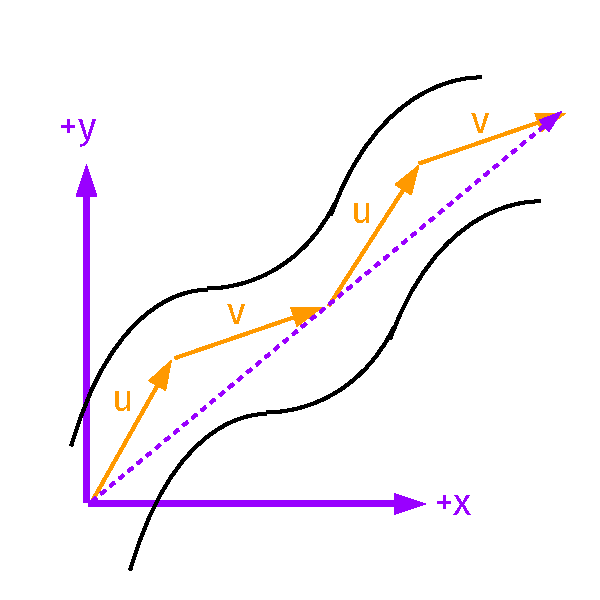
\includegraphics[width=0.52\textwidth]{figures/AveVelocity.pdf}
\caption{\label{fig:avevel} A Formula-1 driver keeps his car on the track by following a path approximated by the position vectors $u$, $v$, $u$, and $v$.  The dashed arrow represents the total displacement.}
\end{figure}
\end{frame}

\begin{frame}{Coordinates and Vectors - Average Velocity (Chapter 2.3)}
If $\vec{u} = (20\hat{i}+30\hat{j})$ m, and $\vec{v} = (30\hat{i}+20\hat{j})$ m, what is the total displacement?  If the elapsed time is 10 seconds, what is the magnitude of the average velocity? \\
\vspace{0.2cm}
\begin{itemize}
\item A: $(50\hat{i} + 50\hat{j})$ m, 14 m/s
\item B: $(80\hat{i} + 100\hat{j})$ m, 10 m/s
\item C: $(100\hat{i} + 100\hat{j})$ m, 14 m/s
\item D: $(50\hat{i} + 150\hat{j})$ m, 10 m/s
\end{itemize}
\end{frame}

\begin{frame}{Coordinates and Vectors (Chapters 3.1 - 3.3)}
PhET simulation about vector addition: \\
\url{https://phet.colorado.edu/en/simulation/vector-addition}
\end{frame}

\section{Kinematics and Newton's Laws}

\begin{frame}{Kinematics and Newton's Laws}
\small
\textit{Kinematics} - A \alert{description} of the motion of particles and systems \\
\textit{Dynamics} - An \alert{explanation} of the motion of particles and systems \\
\vspace{0.25cm}
What causes an object to move?  \textbf{Forces}.  Forces exist as a result of the \alert{\textbf{interactions}} of objects or systems.\\
\vspace{0.25cm}
\rule{10cm}{0.4pt} \\
\vspace{0.25cm}
\textit{Evolution} - A \alert{description} of the change of biological species \\
\textit{Natural Selection} - An \alert{explanation} of change in biological species \\
\vspace{0.25cm}
What causes species to evolve?  \textbf{Natural selection}.  Natural selection exists because of \alert{selection pressures}, \alert{numerous offspring}, and \alert{variation} among offspring.
\end{frame}

\begin{frame}{Kinematics and Newton's Laws}
\textbf{Newton's First Law}: A man slides a palette crate across a concrete floor of his shop.  He exerts a force of 60.0 N, and the box has a constant velocity of 0.5 m/s.  What force cancels his pushing force, and what is the value in Newtons?
\begin{itemize}
\item A: wind, 60.0 N
\item B: friction: 60.0 N
\item C: friction: -60.0 N
\item D: weight: -60.0 N
\end{itemize}
\end{frame}

\begin{frame}{Kinematics and Newton's Laws}
\textbf{Newton's Second Law}: The crate has a mass of 50 kg, and encounters an area where there is no longer friction.  If the pushing force is still 60 N, what is the acceleration?
\begin{itemize}
\item A: 1.0 m/s$^2$
\item B: 0.8 m/s
\item C: 1.2 m/s
\item D: 1.2 m/$^2$
\end{itemize}
\end{frame}

\begin{frame}{Kinematics and Newton's Laws}
\textbf{Kinematics}: If the acceleration is 1.2 m/s$^2$, and the crate begins with a velocity of 1 m/s, what is the velocity after 5 seconds?
\begin{itemize}
\item A: 4 m/s
\item B: 5 m/s
\item C: 6 m/s
\item D: 7 m/s
\end{itemize}
\end{frame}

\begin{frame}{Kinematics and Newton's Laws}
\textbf{Newton's Second Law}: Suppose there is no pushing force, but the crate moves at 5 m/s through an area with a frictional force that has a magnitude of 5 N.  If the crate still weighs 50 kg, what is the acceleration?
\begin{itemize}
\item A: 0.2 m/s$^2$
\item B: -0.1 m/s$^2$
\item C: 1 m/s$^2$
\item D: -2 m/s$^2$
\end{itemize}
\end{frame}

\begin{frame}{Kinematics and Newton's Laws}
\textbf{Newton's Third Law}: If a person hangs from a horizontal rope (with the ends tied to two walls), and the person has a weight $\vec{w} = -600 N$, what is the total upward component of the tension in the rope?
\begin{itemize}
\item A: -600 N
\item B: 60 N
\item C: 600 N
\item D: -60 N
\end{itemize}
\end{frame}

\begin{frame}{Kinematics and Newton's Laws}
\textbf{Newton's Third Law}: If a heavy truck and a light car collide, which exerts the larger force on the other?
\begin{itemize}
\item A: The heavy truck exerts a larger force on the car.
\item B: The light car exerts a larger force on the heavy truck.
\item C: They exert the same force on each other.
\item D: Cannot determine.
\end{itemize}
\end{frame}

\section{Work-Energy Theorem and Conservation of Energy}

\begin{frame}{Kinetic Energy and the Work-Energy Theorem}
\textbf{Group board exercise}: A firework of mass 1 kg is launched straight upwards.  The gunpowder releases 500 J of energy.  What is the velocity of the shell as it leaves the launcher?  How high does it fly straight upwards? \\ \vspace{0.5cm}
Three useful concepts: 1) Work equation 2) Work-energy theorem 3) gravitational potential energy.
\end{frame}

\begin{frame}{Kinetic Energy and the Work-Energy Theorem}
\textbf{Work-energy theorem}: How high in the air would a 0.1 kg rock go if it was launched straight upward by a spring with $k=1000$ N/m, if the spring was compressed $0.1$ m?
\begin{itemize}
\item A: 0.5 m
\item B: 5 m
\item C: 50 m
\item D: 500 m
\end{itemize}
Note: the potential energy of a spring with spring constant $k$ and displacement $x$ is $U = \frac{1}{2}k x^2$.
\end{frame}

\begin{frame}{Kinetic Energy and the Work-Energy Theorem}
\textbf{Work-energy theorem}: How high would it go if the spring was compressed $0.2$ m?
\begin{itemize}
\item A: 100 m
\item B: 200 m
\item C: 500 m
\item D: 50 m
\end{itemize}
Note: think of this exercise as a scaling problem.
\end{frame}

\section{Momentum}

\begin{frame}{Momentum}
A ball with mass 0.1 kg moves at 1 m/s.  It strikes a stationary ball with twice the mass and stops.  The heavier ball moves with a velocity of
\begin{itemize}
\item A: 0.1 m/s
\item B: 1 m/s
\item C: 5 m/s
\item D: 0.5 m/s
\end{itemize}
\end{frame}

\begin{frame}{Momentum}
A ball with mass 0.1 kg moves at 1 m/s.  It strikes a stationary ball with the same mass and they stick together.  What is the final velocity of the object?
\begin{itemize}
\item A: 0.1 m/s
\item B: 1 m/s
\item C: 5 m/s
\item D: 0.5 m/s
\end{itemize}
\end{frame}

\begin{frame}{Momentum}
If the mass of an object that is rotating around an origin with angular velocity $\omega$ decreases by a factor of 2, the new angular velocity will be:
\begin{itemize}
\item A: $-\omega$
\item B: $-3\omega$
\item C: $2\omega$
\item D: $\omega$
\end{itemize}
\end{frame}

\section{Electrostatics I: Chapters 18.1 - 18.5}

\begin{frame}{Electrostatics I - Beginnings}
\small
\begin{figure}
\centering
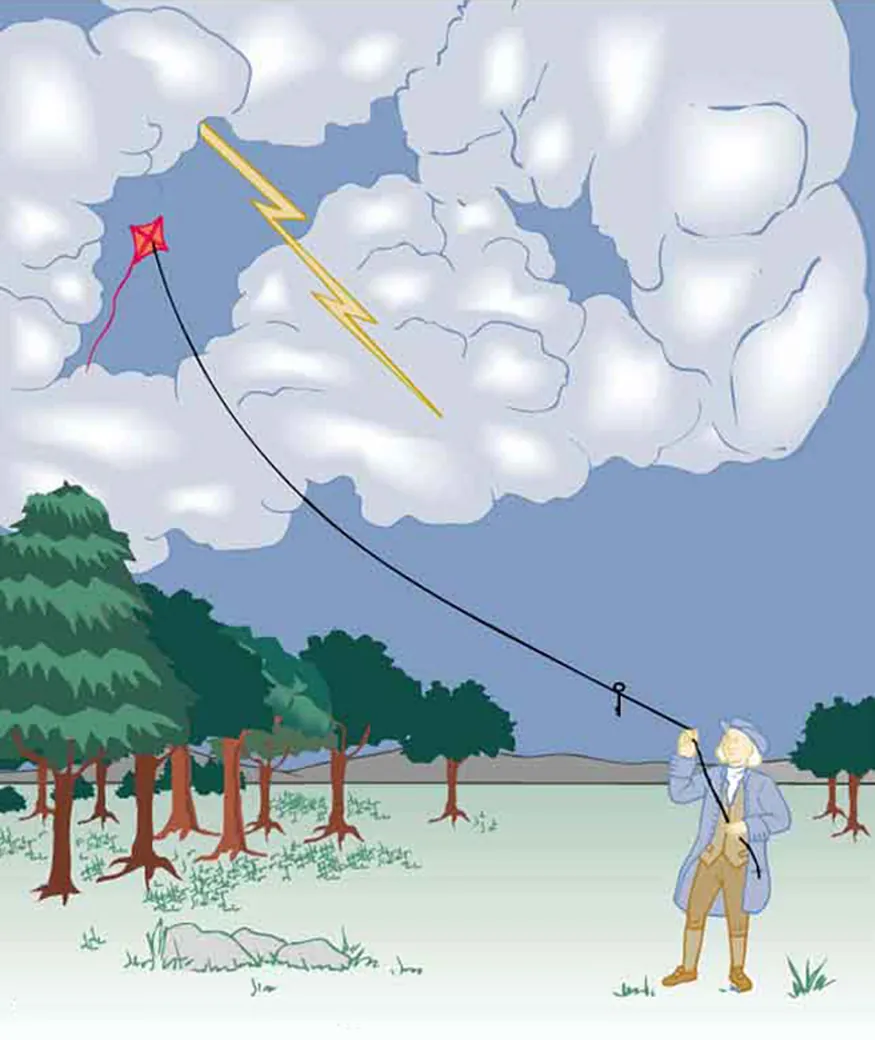
\includegraphics[width=0.18\textwidth]{figures/franklin.png}
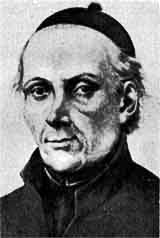
\includegraphics[width=0.15\textwidth]{figures/alzate_ramirez.jpg}
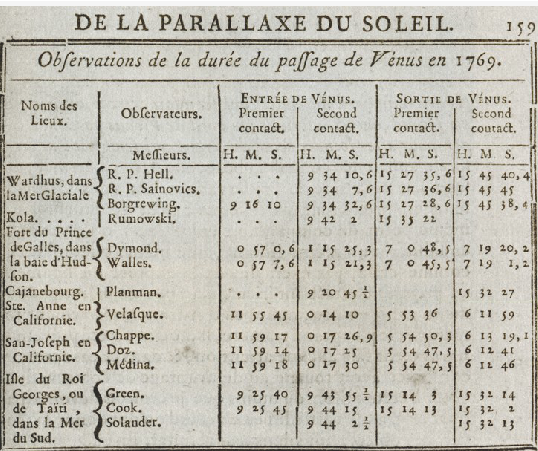
\includegraphics[width=0.26\textwidth]{figures/1769_transit.png}
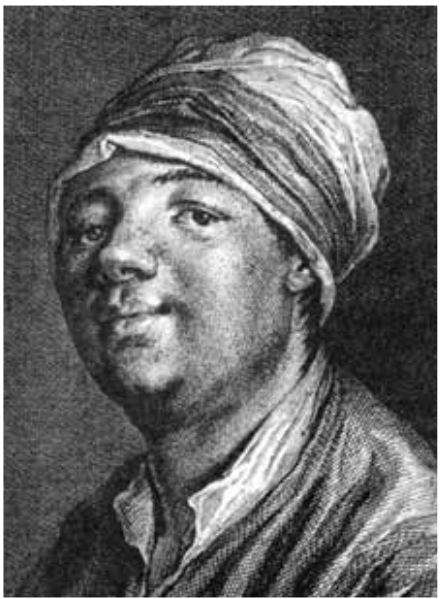
\includegraphics[width=0.16\textwidth]{figures/Abbot_dAuteroche.png}
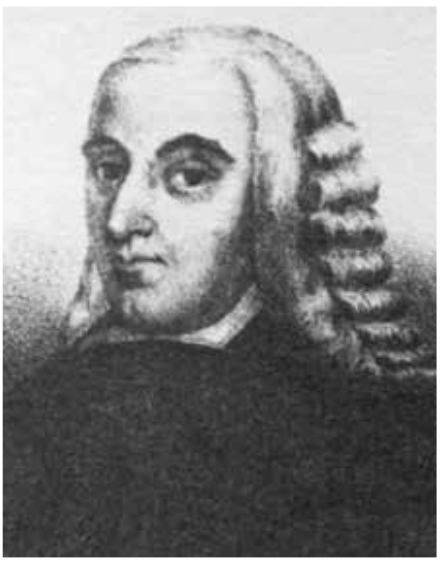
\includegraphics[width=0.17\textwidth]{figures/joaquin_v_d_Leon.png}
\caption{\label{fig:franklin} (a) Benjamin Franklin with kite and key, (b) Father Jos\'{e} Antonio Alzate y Ram\'{i}rez, (c) Table of astronomical data for 1769 Venus transit, (d) Jean-Baptiste Chapp\'{e} d'Auteroche, (e) Joaqu\'{i}n Vel\'{a}zquez de Le\'{o}n.}
\end{figure}
Who first understood the aurora borealis?
\textbf{\alert{\url{https://youtu.be/czMh3BnHFHQ?si=9rd7rpaaUd2Ef_XT}}} \\ \vspace{0.5cm}
Unit 0 concept trailer: \\
\textbf{\alert{\url{https://youtu.be/SglzRDD1oNI}}}
\end{frame}

\begin{frame}{Electrostatics I - Beginnings}
\small
\begin{figure}
\centering
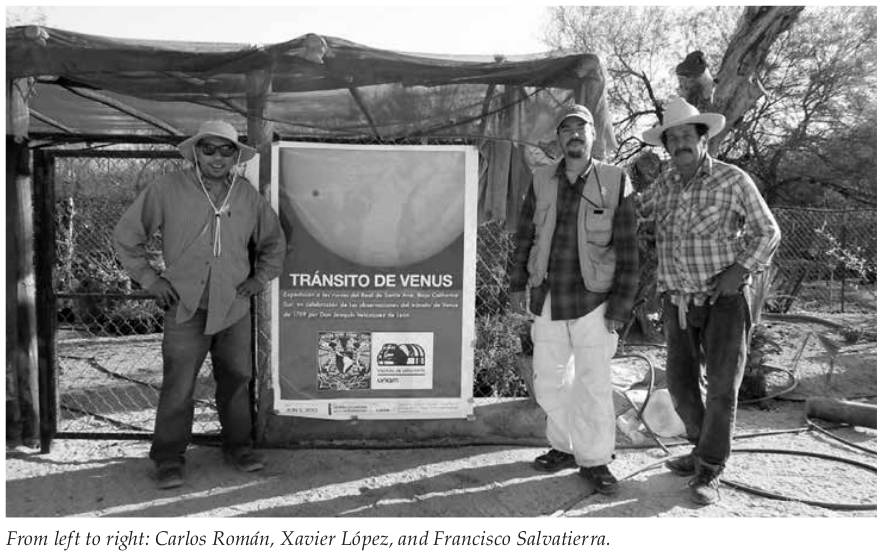
\includegraphics[width=0.55\textwidth]{figures/roman_lopez_salvatierra.png}
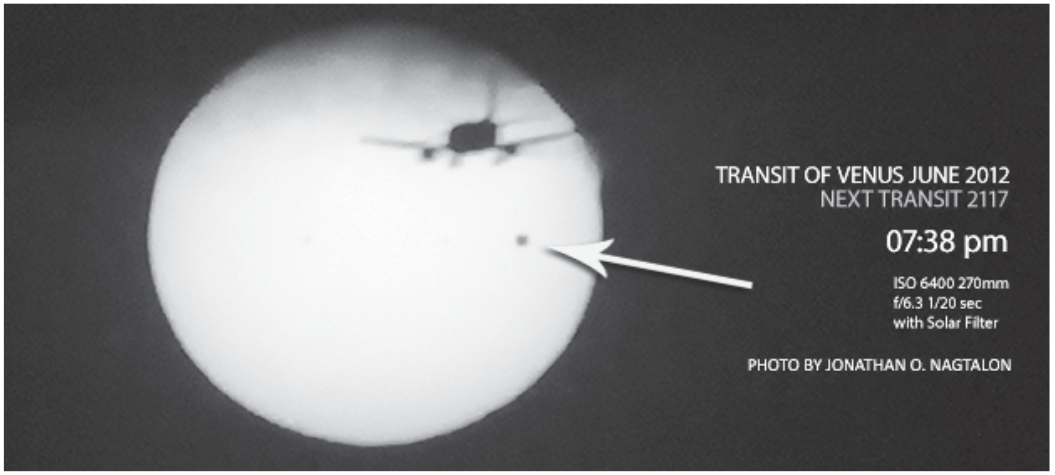
\includegraphics[width=0.55\textwidth]{figures/venus.png}
\caption{\label{fig:franklin2} (Top) Carlos Rom\'{a}n, Xavier L\'{o}pez, and Fransisco Salvatierra. (Bottom) The 2012 Venus transit, from Baja California.}
\end{figure}
\end{frame}

\begin{frame}{Electrostatics I - Applications to Biology}
\begin{figure}
\centering
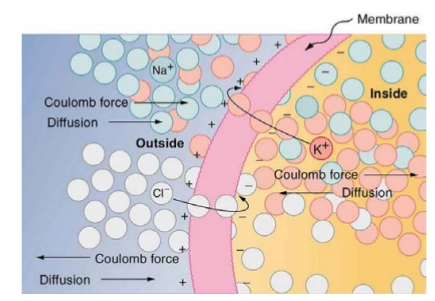
\includegraphics[width=0.45\textwidth]{figures/membrane.png}
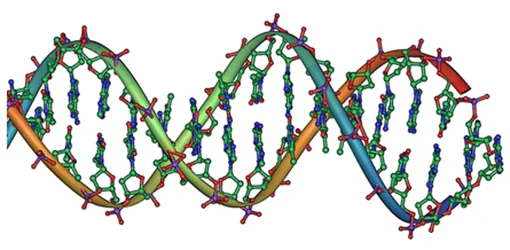
\includegraphics[width=0.45\textwidth]{figures/dna.png}
\caption{\label{fig:membrane} (Left) Nerve signals are caused by electric charge. (Right) The DNA molecule is held together by electrical forces.}
\end{figure}
\end{frame}

\begin{frame}{Electrostatics I - Charge}
\small
\begin{figure}
\centering
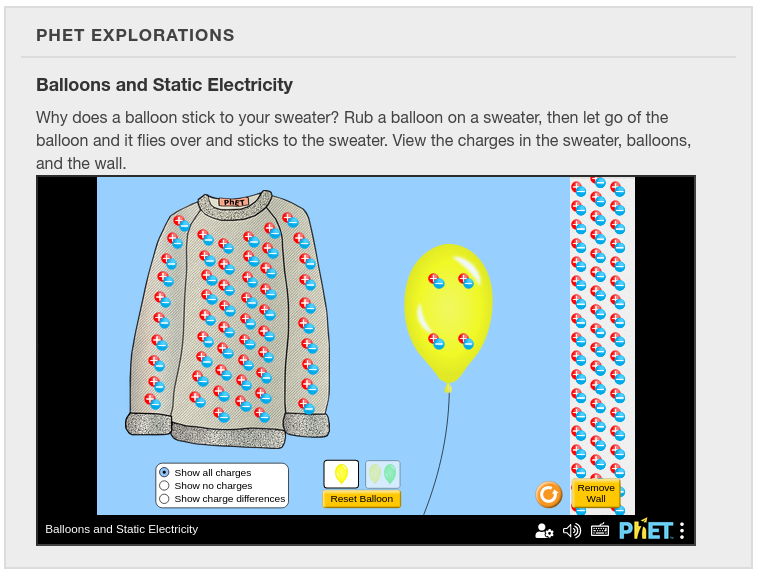
\includegraphics[width=0.5\textwidth]{figures/balloon.png}
\caption{\label{fig:charge1} Convervation of charge: \textbf{\alert{\url{https://phet.colorado.edu/en/simulations/balloons-and-static-electricity}}}.}
\end{figure}
Observations: charge is conserved, there are positive and negative charges, opposite charges attract, like charges repel.  \textit{Can you deduce these without seeing the charges?}
\end{frame}

\begin{frame}{Electrostatics I - Charge}
\begin{itemize}
\item \textbf{Conductors} - These can have net charge, and charge moves around freely.  Consider \textit{the wall} in the balloon example.
\item \textbf{Insulators} - These can have net charge, but charge cannot move freely.  Consider \textit{the balloon} in the previous example.
\item \textbf{Unit of charge} - 1 unit of charge is $q_{\rm e} = 1.60 \times 10^{-19}$ C
\item \textbf{The Coulomb} - 1 C is $0.625 \times 10^{19} q_{\rm e}$
\item \textbf{The Amp\`{e}re (amp)} - 1 Coulomb is 1 amp of current for 1 second.
\end{itemize}
\end{frame}

\subsection{Activity: PhET Simulation of Charges and Fields}

\begin{frame}{Activity: PhET Charges and Fields}
At your tables, go to the following URL: \\ \vspace{0.2cm}
\url{https://phet.colorado.edu/en/simulation/charges-and-fields} \\ \vspace{0.2cm}
Click on the java app to get it running.  Notice the following:
\begin{enumerate}
\item This is a 2D coordinate space, and you can activate the grid lines at right, by clicking \textit{grid.}
\item Clicking \textit{values} gives you the measurement scale.
\item Click \textit{electric field}, or make sure it is activated.
\item Verify the length scale with the \textbf{ruler tool}, shaped like a tape measure.  It can be dragged from the box at right.
\end{enumerate}
\end{frame}

\begin{frame}{Activity: PhET Charges and Fields}
\small
\url{https://phet.colorado.edu/en/simulation/charges-and-fields} \\ \vspace{0.2cm}
\textbf{Click and drag a positive charge into the 2D coordinate system.  This is analagous to charging an insulator.}
\begin{enumerate}
\item Drag the yellow tool at the bottom into the space, and use it to measure the \textit{electric field} $E$.  Notice the units are in V/m and m.  The electric field units V/m are equivalent to Newtons per Coulomb (N/C).
\item Copy to excel the field strength (E) versus distance (r).  Use 25 cm distance increments, and record 15 data points in two columns.
\item In a third column, compute $r^2$.
\end{enumerate}
\end{frame}

\begin{frame}{Activity: PhET Charges and Fields}
\small
\url{https://phet.colorado.edu/en/simulation/charges-and-fields} \\ \vspace{0.2cm}
\textbf{Click and drag a positive charge into the 2D coordinate system.  This is analagous to charging an insulator.}
\begin{enumerate}
\item Plot $E$ vs. $r^2$.  Do you observe a linear trend?  What are some sources of error that contribute to the uncertainty in the slope?
\item Repeat this same exercise, but instead of measuring field strength versus \textit{distance}, measure it in one location, versus \textit{charge.} Take 15 data points in two columns and plot $E$ versus $q$ in Excel.  What is the slope of the line?  Notice the units of charge are nC.
\end{enumerate}
\textbf{Example data:} See Moodle for sample data drawn from this PhET.
\end{frame}

\begin{frame}{Electrostatics I - Coulomb Force}
\textbf{Coulomb's Law} describes the force between charges. \\ \vspace{0.5cm}
\begin{tcolorbox}[colback=white,colframe=gray,title=Coulomb's Law]
\alert{The electric force, or \textbf{Coulomb force}, between two electrically charged systems with charges $q_{\rm 1}$ and $q_{\rm 2}$ separated by a distance $r$ is
\begin{equation}
\vec{F}_{\rm C} = \frac{1}{4\pi\epsilon_{\rm 0}} \frac{q_{\rm 1} q_{\rm 2}}{r^2} \hat{r} \label{eq:C}
\end{equation}
In Eq. \ref{eq:C}, $\hat{r} = \vec{r}/|\vec{r}|$, and $\epsilon_{\rm 0} = 8.85418782\times 10^{-12} N^{-1} m^{-2} C^2$, called the \textit{perimittivity of free space.}}
\end{tcolorbox}
\end{frame}

\begin{frame}{Electrostatics I - Coulomb Field}
\begin{tcolorbox}[colback=white,colframe=gray,title=Coulomb Field]
\alert{The electric field corresponding to Eq. \ref{eq:C}, experienced by a charge $q$ and generated by a charge $Q$ is 
\begin{equation}
\vec{E}_{\rm C} = \frac{1}{4\pi\epsilon_{\rm 0}} \frac{Q}{r^2} \hat{r} \label{eq:Cf}
\end{equation}
In Eq. \ref{eq:Cf}, $r$ remains the separation between $q$ and $Q$.}
\end{tcolorbox}
Thus we have: $\vec{F}_{\rm C} = q \vec{E}_{\rm C}$.
\end{frame}

\begin{frame}{Electrostatics I - Coulomb Force}
Suppose a charge $+q$ experiences the Coulomb field of another charge of $-q$, separated by a distance $r$.  Which of the following is true?
\begin{itemize}
\item A: The charge $+q$ accelerates the $-q$ charge only.
\item B: The charge $-q$ accelerates the $+q$ charge only.
\item C: No charges move; the force on one is equal to the force on the other.
\item D: Both charges move, and the force on one is equal to the force on the other.
\end{itemize}
\end{frame}

\begin{frame}{Electrostatics I - Coulomb Force}
Recall Newton's Third Law:
\begin{figure}
\centering
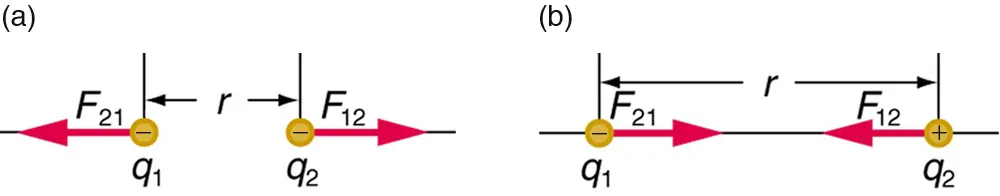
\includegraphics[width=0.9\textwidth]{figures/third.png}
\caption{\label{fig:third} Newton's Third Law still applies to the electrostatic force.}
\end{figure}
\end{frame}

\begin{frame}{Electrostatics I - Coulomb Field}
\small
\begin{columns}[T]
\begin{column}{0.5\textwidth}
What is the angle of the E-field at point (1,1) in Fig. \ref{fig:netfield2} at right?
\begin{itemize}
\item A: 0 deg
\item B: 45 deg
\item C: 90 deg
\item D: 135 deg
\end{itemize}
What is the fastest way to solve this problem?
\begin{itemize}
\item A: Guess
\item B: Guess harder
\item C: Lots of algebra
\item D: Symmetry
\end{itemize}
\end{column}
\begin{column}{0.5\textwidth}
\begin{figure}
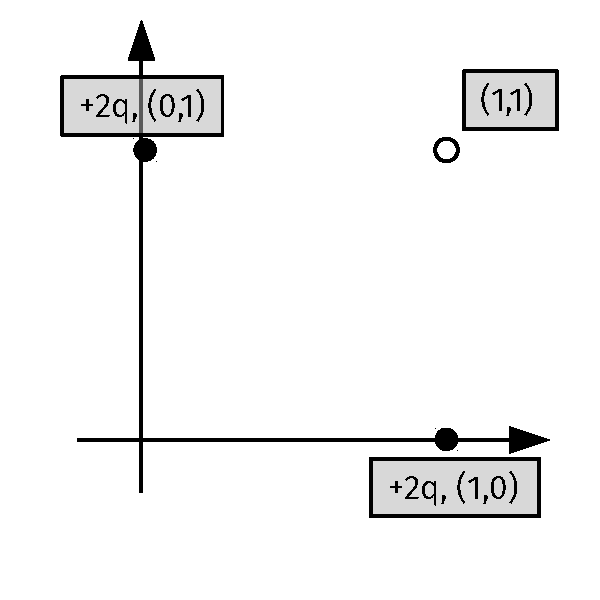
\includegraphics[width=\textwidth]{figures/NetField2.pdf}
\caption{\label{fig:netfield2} Two charges create a field for a hypothetical \textit{test charge}.}
\end{figure}
\end{column}
\end{columns}
\end{frame}

\begin{frame}{Electrostatics I - Coulomb Field}
\small
\begin{columns}[T]
\begin{column}{0.5\textwidth}
Which of the following is true of the E-field at point (1,1) in Fig. \ref{fig:netfield3} at right?
\begin{itemize}
\item A: The angle with respect to the x-axis is 45 degrees
\item B: The angle with respect to the x-axis is greater than 45 degrees
\item C: The angle with respect to the x-axis is less than 45 degrees
\item D: The angle with respect to the x-axis is 90 degrees
\end{itemize}
\end{column}
\begin{column}{0.5\textwidth}
\begin{figure}
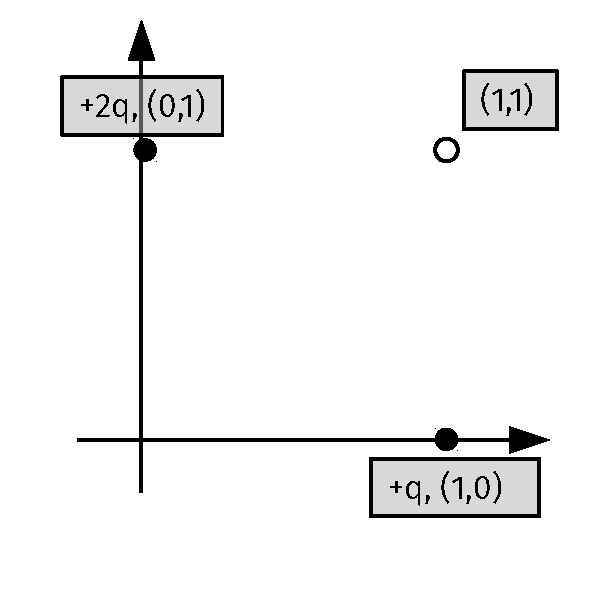
\includegraphics[width=\textwidth]{figures/NetField3.pdf}
\caption{\label{fig:netfield3} Two charges create a field for a hypothetical \textit{test charge}.}
\end{figure}
\end{column}
\end{columns}
\end{frame}

\begin{frame}{Electrostatics I - Coulomb Field}
The forces of $N$ fixed charges on a test charge $q$ create a net force, where the individual forces simply add like vectors.  This is known as the \textbf{superposition principle}.
\begin{tcolorbox}[colback=white,colframe=gray,title=Superposition Principle]
\begin{align}
\vec{F}_{\rm C,Net} &= \frac{1}{4\pi\epsilon_{\rm 0}} q \sum_{i = 1}^N \frac{q_i}{r_i^2}\hat{r}_i = q \vec{E}_{\rm C,Net} \\
\vec{E}_{\rm C,Net} &= \frac{1}{4\pi\epsilon_{\rm 0}} \sum_{i = 1}^N \frac{q_i}{r_i^2}\hat{r}_i
\end{align}
\end{tcolorbox}
\textbf{Short PhET demonstration}: create a circle of charges, and determine the field at the center.
\end{frame}

\begin{frame}{Electrostatics I - Coulomb Field}
\small
\begin{columns}[T]
\begin{column}{0.5\textwidth}
The following problem is an example of solving for a field analytically, and \textit{testing various limits}.  Upon taking limits results are often simple and intuitive. \\ \vspace{0.5cm}
Two charges $+q$ are on the fixed in an insulator on the x-axis.  Solve for the E-field at $P = (0,0,z)$. \\ \vspace{0.5cm}
(Professor demonstrate on board).
\begin{equation}
\vec{E}(z) = \frac{1}{4\pi\epsilon_0} \frac{2qz}{\left(z^2+\left(\frac{d}{2}\right)^2\right)^{3/2}} \hat{k}
\end{equation}
\end{column}
\begin{column}{0.5\textwidth}
\begin{figure}
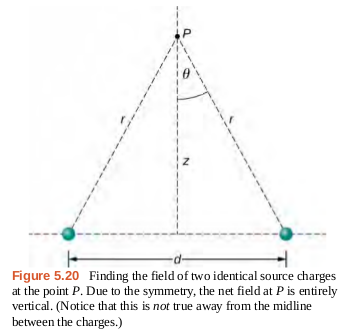
\includegraphics[width=\textwidth]{figures/twoChargesZ.png}
\caption{\label{fig:twoChargesZ} Solve for the E-field as a function of $z$, $d$, and $q$.}
\end{figure}
\end{column}
\end{columns}
\end{frame}

\begin{frame}{Electrostatics I - Coulomb Field}
\small
\begin{columns}[T]
\begin{column}{0.5\textwidth}
Show that the general solution is
\begin{equation}
\vec{E}(z) = \frac{1}{4\pi\epsilon_0} \frac{2qz}{\left(z^2+\left(\frac{d}{2}\right)^2\right)^{3/2}} \hat{k}
\end{equation}
\textit{Take the following two limits:} \\ 1) $z \gg d$ and 2) $z=0$.  What are the results? \\ \vspace{0.5cm}
Keep these results in mind, because we are about to start drawing \textbf{vector fields,} in order to visualize the algebra.
\end{column}
\begin{column}{0.5\textwidth}
\begin{figure}
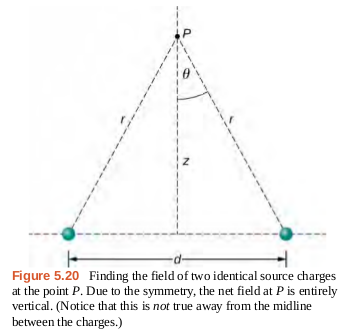
\includegraphics[width=\textwidth]{figures/twoChargesZ.png}
\caption{\label{fig:twoChargesZ2} Solve for the E-field as a function of $z$, $d$, and $q$.}
\end{figure}
\end{column}
\end{columns}
\end{frame}

\subsection{Activity: PhET Simulation of Charges and Fields}

\begin{frame}{Activity: PhET Charges and Fields}
\textbf{PhET Simulation of E-fields from Charges}: \\ \vspace{0.5cm}
\url{https://phet.colorado.edu/en/simulation/charges-and-fields}
\begin{enumerate}
\item Create the situation in the prior problem, in Fig. \ref{fig:twoChargesZ2}.
\item Use the yellow sensor object to determine the local direction of the E-field at various points along the z-axis.
\begin{itemize}
\item Do the results match the limit $z\gg d$?
\item Do the results match the limit $z = 0$, halfway between the charges?
\item Where is the field maximal?
\end{itemize}
\item Make sure you can see above and below the charges, and repeat steps 1 and 2 for negative z-values.  What do you find?
\end{enumerate}
\end{frame}

\section{Electrostatics II: Chapters 19.1 - 19.3}

\begin{frame}{Electrostatics II - Potential and Potential Energy}
Recall that the \textit{change in potential energy} is force:
\begin{equation}
F = -\frac{\Delta U}{\Delta x}
\end{equation}
\begin{itemize}
\item The units of $U$: Joules = Newtons per meter
\item The units of $x$: meters
\item The ratio: Newtons
\end{itemize}
\textbf{Instructor examples:} (a) force of gravity near surface of Earth, (b) force of spring.
\end{frame}

\begin{frame}{Electrostatics II - Potential and Potential Energy}
The negative change in potential energy gives us the force.  Often in electrostatics, we just need the electric field.  The negative change in the \textit{potential} gives us the field, because we just factor out the test charge:
\begin{align}
F &= -\frac{\Delta U}{\Delta x} =  -\frac{q\Delta V}{\Delta x}\\
E &= F/q = -\frac{\Delta V}{\Delta x} \label{eq:volt}
\end{align}
In Eq. \ref{eq:volt}, we refer to $\Delta V$ as \textbf{voltage}.  Voltage is the potential energy per unit charge.
\end{frame}

\subsection{Activity: PhET Simulation of Charges and Fields}

\begin{frame}{Activity: PhET Simulation of Charges and Fields}
\small
\url{https://phet.colorado.edu/en/simulation/charges-and-fields} \\
\begin{enumerate}
\item Place a positive charge, and measure the voltage with the blue tool at right.
\item Voltage should be a \textit{number}, not a \textit{vector.}
\item Measure the voltage in 25 cm increments for 15 data points, and copy the data to Excel.  One column should be the distance $r$ in meters, and the other column should be the voltage $V$ in \textbf{Volts.}
\item Plot the data in Excel, and fit a \textit{power-law} trendline to the data.  What do you notice?
\item Plot $V$ vs. $r^{-1}$.  What do you notice?
\end{enumerate}
\end{frame}

\begin{frame}{Activity: PhET Simulation of Charges and Fields}
Same PhET simulation:
\begin{enumerate}
\item Measure the voltage from the same charge and tool position (fixed $r$), but vary the \textit{amount of charge.}
\item Take 15 measurements, adding a positive red charge each time.
\item Plot the voltage in \textbf{Volts} vs. the charge in nano-Coulombs (nC).  What do you notice?
\end{enumerate}
\end{frame}

\begin{frame}{Electrostatics II - Potential of a Point Charge}
\begin{tcolorbox}[colback=white,colframe=gray,title=Potential of a Point Charge]
The potential a distance $r$ from a charge $q$ is given by
\begin{equation}
\boxed{
V = \frac{1}{4\pi \epsilon_0} \frac{q}{r}} \label{eq:volt2}
\end{equation}
\end{tcolorbox}
If a potential of 4 Volts is felt a distance of 0.1 m from a charge q, what is the potential at 0.4 m?
\begin{itemize}
\item A: 5 Volts
\item B: 4 Volts
\item C: 3 Volts
\item D: 2 Volts
\end{itemize}
\end{frame}

\begin{frame}{Electrostatics II - Potential of a Point Charge}
\begin{tcolorbox}[colback=white,colframe=gray,title=Potential of a Point Charge]
The potential a distance $r$ from a charge $q$ is given by
\begin{equation}
\boxed{
V = \frac{1}{4\pi \epsilon_0} \frac{q}{r}}
\end{equation}
\end{tcolorbox}
If a potential of 3 Volts is felt a distance of 3 m from a charge q, what is the potential at 1 m?
\begin{itemize}
\item A: 1 Volts
\item B: 3 Volts
\item C: 6 Volts
\item D: 9 Volts
\end{itemize}
\end{frame}

\subsection{Activity: PhET Simulation of Charges and Fields}

\begin{frame}{Activity: PhET Simulation of Charges and Fields}
Create the system shown in Fig. \ref{fig:cap_phet} in the PhET simulator \textit{Charges and Fields}.  The lines of charge should be far enough apart to allow several measurement locations, but close enough for the superposition principle to matter.
\begin{figure}
\centering
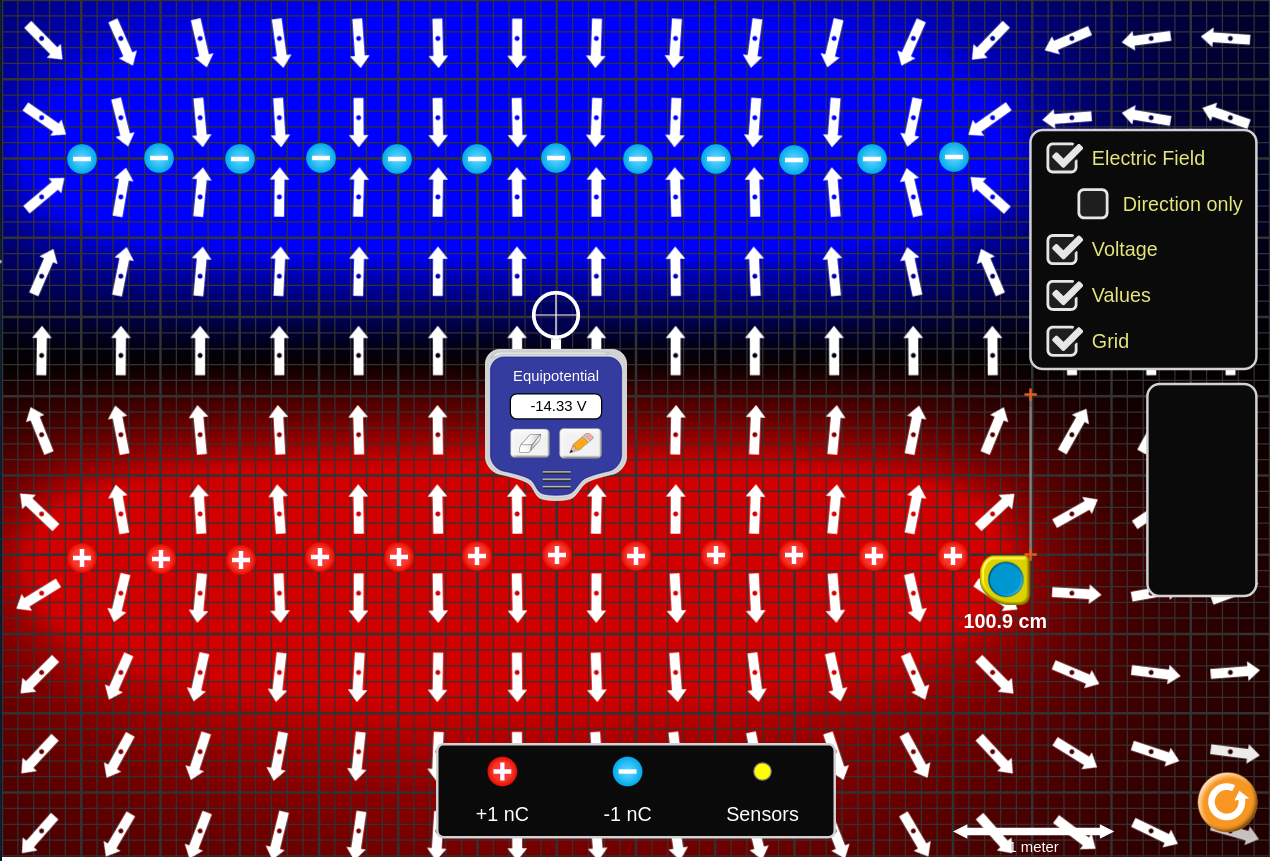
\includegraphics[width=0.5\textwidth]{figures/cap.png}
\caption{\label{fig:cap_phet} Parallel rows of positive and negative charges.  The voltage button illustrates positive voltage in red, and negative voltage in blue.}
\end{figure}
\end{frame}

\begin{frame}{Activity: PhET Simulation of Charges and Fields}
\small
\url{https://phet.colorado.edu/en/simulation/charges-and-fields} \\
\begin{enumerate}
\item Measure the voltage in 10 cm increments for 10-15 data points, and copy the data to Excel.  One column should be the distance $r$ in meters, and the other column should be the voltage $V$ in Volts.
\item Plot the data and fit a \textit{linear} trendline to the data.  Is the model a good fit?
\item \textbf{\alert{Key question:}} if the voltage depends linearly on the displacement, how does the E-field depend on displacement?
\item The system we have created is known as a \textit{capacitor.}
\end{enumerate}
\end{frame}

\begin{frame}{Electrostatics II - Potential of Capacitor}
\small
\begin{columns}[T]
\begin{column}{0.5\textwidth}
Suppose the potential across the parallel-plate capacitor in Fig. \ref{fig:cap2} is 12 Volts.  If a $q = +1$ nC charge is released at the positive side, and pops out from a hole on the negative side, what kinetic energy will $q$ have?
\begin{itemize}
\item A: -12 nJ
\item B: 0 nJ
\item C: 12 nJ
\item D: 12 J
\end{itemize}
\footnotesize
Remember: $\Delta V$ is the potential energy \textit{per unit charge,} so $\Delta U = q \Delta V$, and $E = -\Delta V / \Delta x$.
\end{column}
\begin{column}{0.275\textwidth}
\begin{figure}
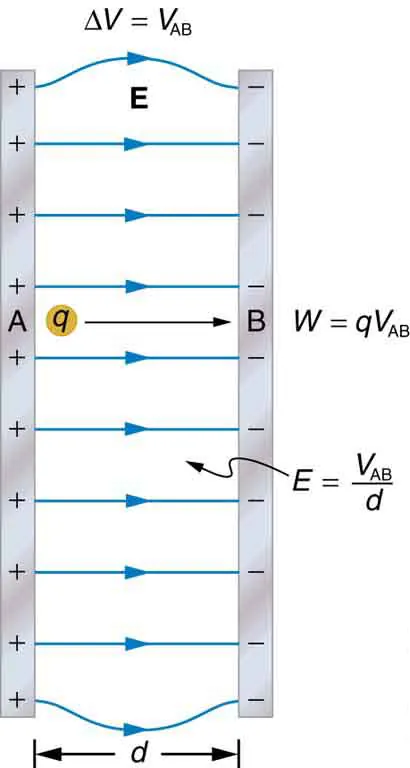
\includegraphics[width=\textwidth]{figures/cap2.png}
\caption{\label{fig:cap2} A capacitor with $\Delta V = 12$ V.}
\end{figure}
\end{column}
\end{columns}
\end{frame}

\begin{frame}{Electrostatics II - Potential of Capacitor}
\small
\begin{columns}[T]
\begin{column}{0.5\textwidth}
If the plates of charge in Fig. \ref{fig:cap3} are separated by 1 mm, what is the value of the electric field?
\begin{itemize}
\item A: -12 V/mm
\item B: 0 V/mm
\item C: 12 V/m
\item D: 12 V/mm
\end{itemize}
\footnotesize
Remember: $\Delta V$ is the potential energy \textit{per unit charge,} so $\Delta U = q \Delta V$, and $E = -\Delta V / \Delta x$.
\end{column}
\begin{column}{0.275\textwidth}
\begin{figure}
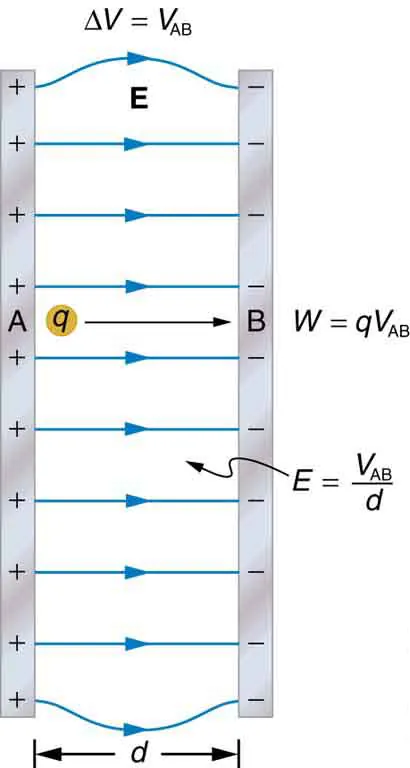
\includegraphics[width=\textwidth]{figures/cap2.png}
\caption{\label{fig:cap3} A capacitor with $\Delta V = 12$ V.}
\end{figure}
\end{column}
\end{columns}
\end{frame}

\begin{frame}{Electrostatics II - Potential of Capacitor}
\small
\begin{columns}[T]
\begin{column}{0.5\textwidth}
There is a difference between a \textit{capacitor} and a \textit{battery} that we will understand soon.  For now, assume Fig. \ref{fig:cap4} represents a 12 V battery, and the total charge is 3600 C.  If we connect a 36 Watt light to the voltage, how long before all the charge is gone?
\begin{itemize}
\item A: 1 minute
\item B: 20 minutes
\item C: 1 hour
\item D: 12 hours
\end{itemize}
\footnotesize
Remember that 1 Watt is 1 Joule per second.
\end{column}
\begin{column}{0.275\textwidth}
\begin{figure}
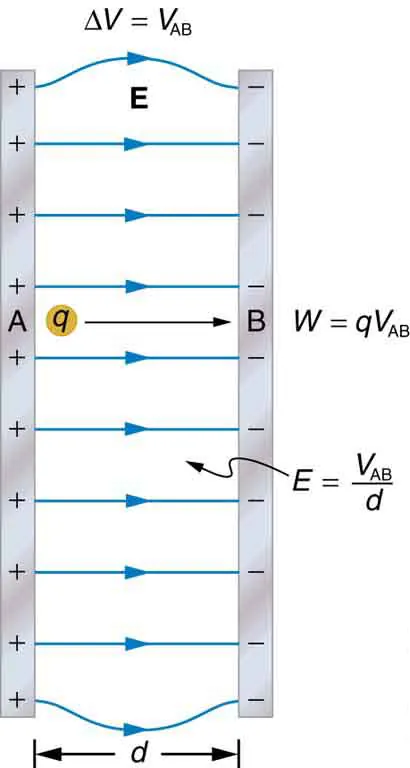
\includegraphics[width=\textwidth]{figures/cap2.png}
\caption{\label{fig:cap4} A capacitor with $\Delta V = 12$ V.}
\end{figure}
\end{column}
\end{columns}
\end{frame}

\section{Applications of Electrostatics in Biology I}

\begin{frame}{Applications of Electrostatics in Biology I}
\small
\begin{columns}[T]
\begin{column}{0.5\textwidth}
\begin{figure}
\centering
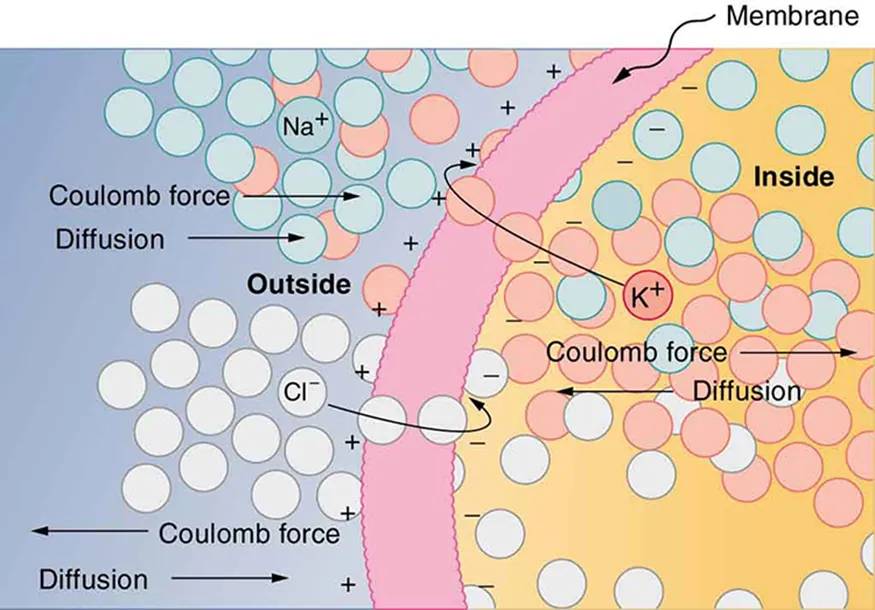
\includegraphics[width=0.75\textwidth]{figures/cell_wall.png} \\
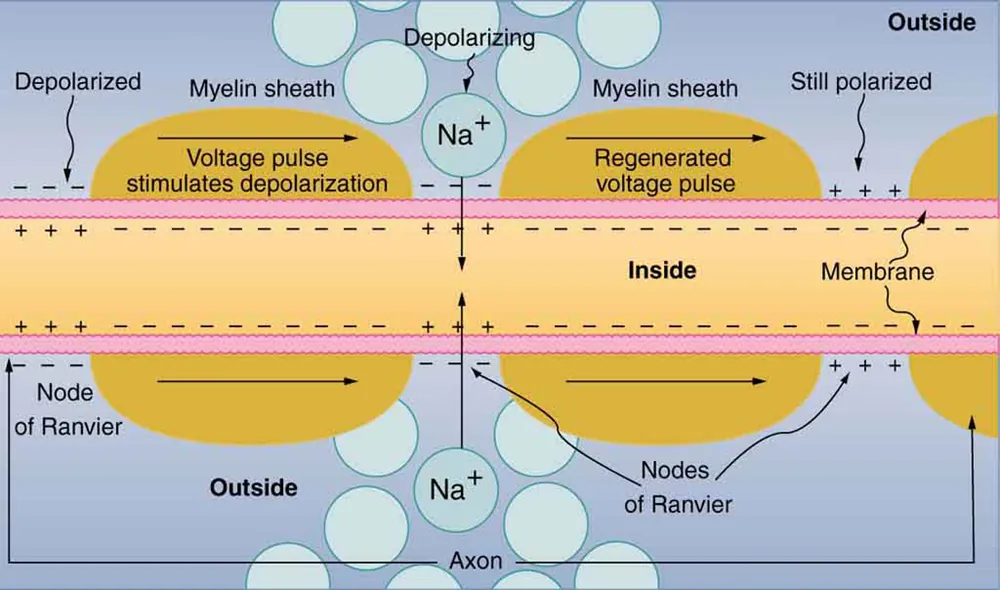
\includegraphics[width=0.75\textwidth]{figures/cell_wall_2.png}
\caption{\label{fig:nerve_a} (Top) Nerve cell membrane (Bottom) Axon membrane with myelin sheath, and nodes.}
\end{figure}
\end{column}
\begin{column}{0.5\textwidth}
\begin{figure}
\centering
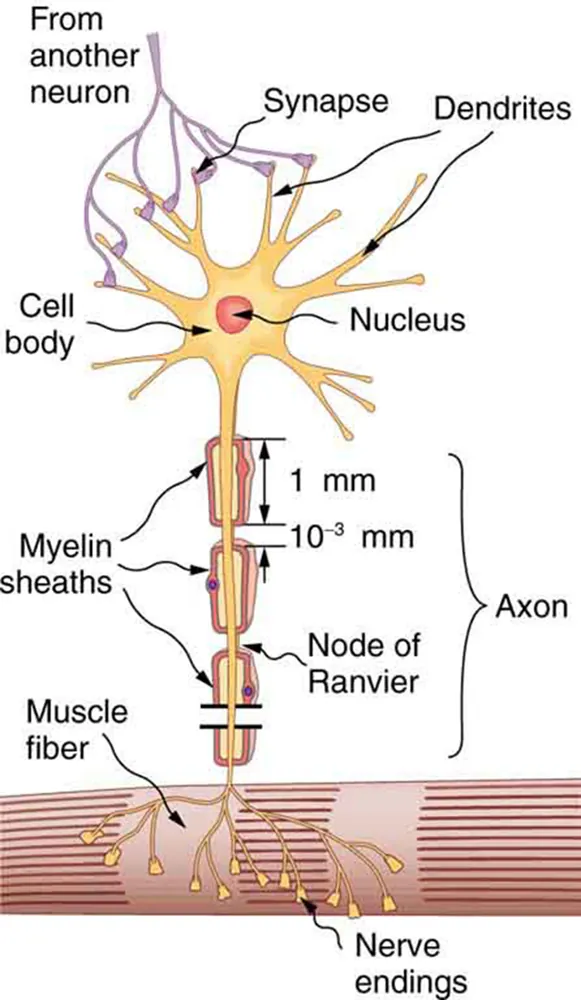
\includegraphics[width=0.65\textwidth]{figures/neuron.png}
\caption{\label{fig:nerve_b} The general structure of a neuron.}
\end{figure}
\end{column}
\end{columns}
\end{frame}

\begin{frame}{Applications of Electrostatics in Biology I}
\begin{figure}
\centering
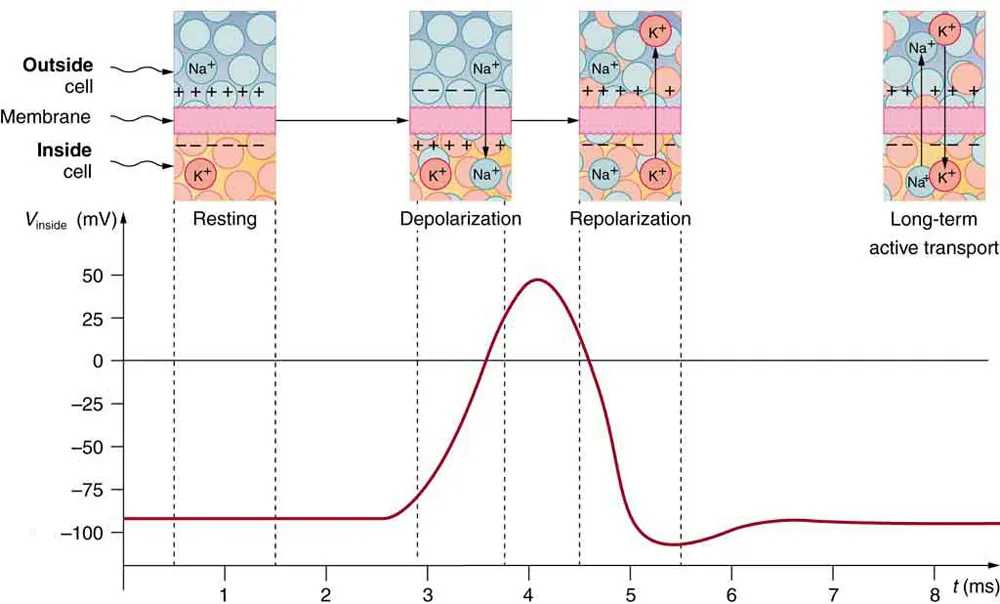
\includegraphics[width=0.8\textwidth]{figures/cell_wall_graph.png}
\caption{\label{fig:nerve2} There are four stages to nerve signal propagation: resting, depolarization, repolarization, and long-term active transport.}
\end{figure}
\end{frame}

\begin{frame}{Applications of Electrostatics in Biology I}
\small
\begin{columns}[T]
\begin{column}{0.5\textwidth}
\begin{figure}
\centering
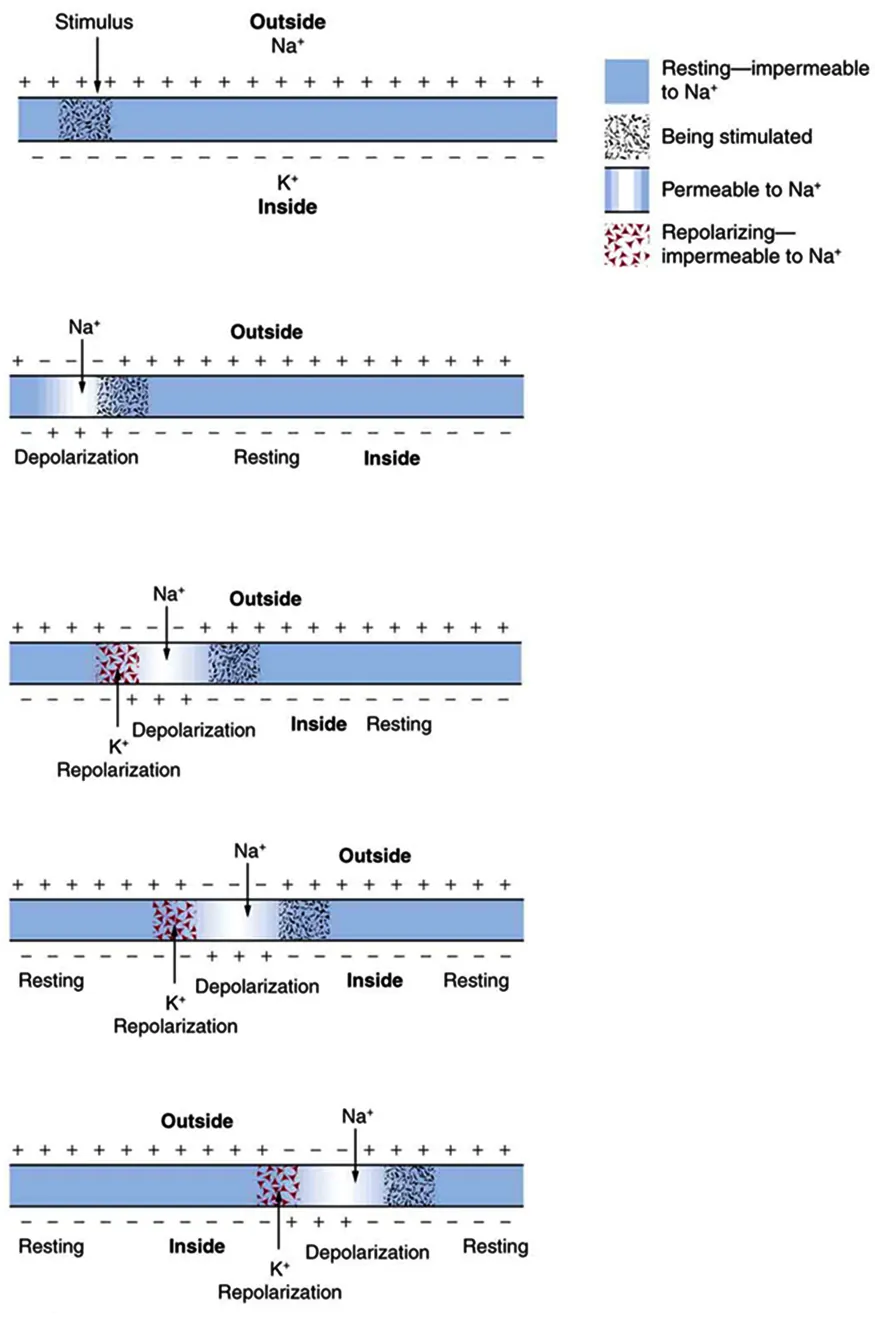
\includegraphics[width=0.85\textwidth]{figures/nerve_prop.png}
\caption{\label{fig:nerve3}}
\end{figure}
\end{column}
\begin{column}{0.5\textwidth}
\textbf{Signal propagation}
\begin{itemize}
\item Stimulus causes Na-ion permeability
\item Na-ions depolarize membrane
\item Depolarization starts depolarization in adjacent area
\end{itemize}
\textbf{Return to equilibrium}
\begin{itemize}
\item Repolarization begins at original location
\item Each area that is depolarized repolarizes, but in the order stimulated
\end{itemize}
\end{column}
\end{columns}
\end{frame}

\begin{frame}{Applications of Electrostatics in Biology I}
\small
PhET simulation of the cell membrane: \\ \url{https://phet.colorado.edu/en/simulations/neuron}
\begin{figure}
\centering
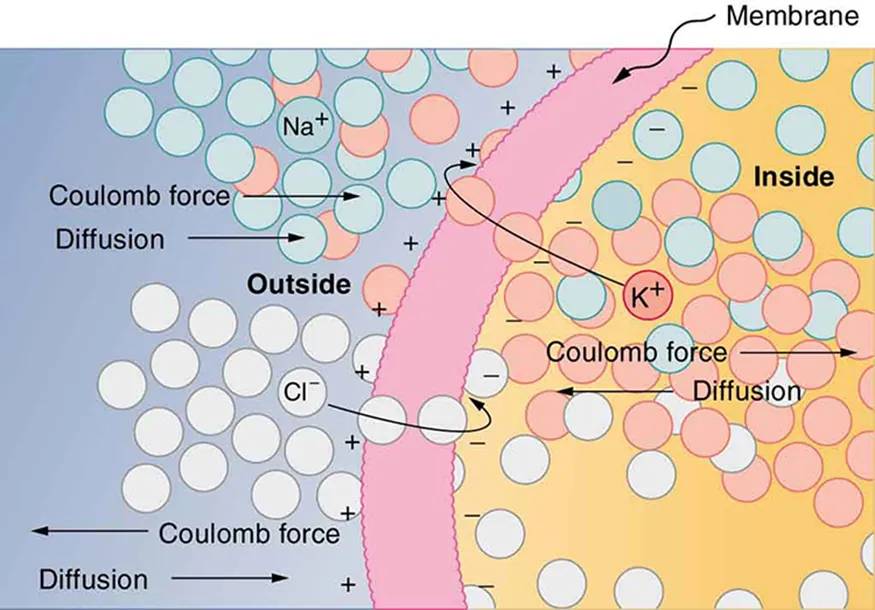
\includegraphics[width=0.6\textwidth]{figures/cell_wall.png}
\caption{\label{fig:nerve4} We can model this process and study the electrical and physiological implications.}
\end{figure}
\end{frame}

\section{Conclusion}

\begin{frame}{Unit 0 Summary}
\textbf{Reading: Chapters 3.1 - 3.3, 18.1 - 18.5, 19.1 - 19.3}
\begin{enumerate}
\item Estimation/Approximation
\item Coordinates and Vectors
\item Review of concepts from Newtonian mechanics
\begin{itemize}
\item Kinematics and Newton's Laws
\item Work-energy theorem, energy conservation
\item Momentum, conservation of momentum
\end{itemize}
\item Electrostatics I: charges and fields
\item Electrostatics II: potential, and potential energy
\end{enumerate}
\end{frame}

\end{document}
